\chapter{Background} \label{background}

In this chapter, we will look at the fundamental concepts and background information for the different diffusion model, the seed selection problem and performing breadth-first search using matrix multiplication. We will also have a look at High Level synthesis and Information about the zedboard. This chapter will contain notations that we will use throughout the report. One aspect we will focus on, is how we can perform graph algorithm such as breadth first search as matrix multiplication. The motivation for transforming breadth first search as matrix-vector multiplication is that displaying the graph algorithm as a matrix multiplication can display the data access pattern for the algorithm and can be readily optimized  \cite{AlgoToMath}. We will look at the independent cascade model, which is a special case of breadth first search  \cite{HybridBFS2015}. By looking at how to improve BFS, we can apply such optimization to ICM and the seed selection algorithm. Another major part of the report is to utilize High Level Synthesis to synthesise the algorithm. \\

\begin{figure}[!ht]
	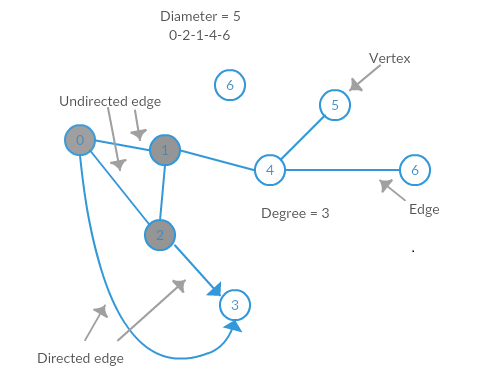
\includegraphics[scale=0.7]{Figures/smallExampleNetwork2}
	\caption{Simple network} 
	\label{fig:SimpleGraph}
\end{figure}

\section{Network teminalogy and glossary}
The fundamental unit in a network is a \textit{vertex} (pl. vertices), sometimes called a node. For this report, both vertex and node will be used. The "bridge" or the line connecting two vertices is called an \textit{edge}, and is shown in Figure \ref{fig:SimpleGraph}.  Different networks have different types of edges, some are\textit{directed}, while others are \textit{undirected}. A directed edge is an edge that runs in only one direction (such as a one-way road between two points), and undirected runs in both directions. Directed edges can be thought of as sporting arrows indicating their orientation, while undirected edges have no such orientation. A graph is directed if all of its edges are directed.

Each vertex has a value that is called \textit{degree}. Degree for a vertex $v_1$ is the amount of edges connected to $v_1$. Note that the degree is not necessarily equal to the number of vertices adjacent to a vertex, since there may be more than one edge between any two vertices. A directed graph has both an in-degree and an out-degree for each vertex, which are the numbers of in-coming and out-going edges respectively. The \textit{component} to which a vertex belongs is that set of vertices that can be reached from it by paths running along edges of the graph. In a directed graph a vertex has both an in-component and an out-component, which are the sets of vertices from which the vertex can be reached and which can be reached from it.

A \textit{geodesic path} is the shortest path through the network from one vertex to another. Note that there may be and often is more than one geodesic path between two vertices. The \textit{diameter} of a network, however,  is the length (in number of edges) of the longest geodesic path between any two vertices. A few authors have also used this term to describe the average geodesic distance in a graph, although strictly the two quantities are quite distinct.

\section{Network}
A \textit{network} is a collection of vertices and edges  \cite{ComplexNetwork2003}. In the real world, multiple systems takes the form of networks around the world, examples are the internet, the World Wide Web, social media like Facebook, Twitter etc.  There are different types of network. These include  \textit{social network} \cite{ComplexNetwork2003}, \textit{information networks} \cite{ComplexNetwork2003}, \textit{technological networks} \cite{ComplexNetwork2003} ,and \textit{biological network} \cite{ComplexNetwork2003}. Different network have different properties and in this report we will look at those most relevant to social networks.

\subsection{Social network}
A social network is a set of individuals connected to each other via some form of contact or interactions \cite{ComplexNetwork2003}. The nodes are people while the edges are the connections between people. The social network display information regarding connection, interaction or location of a set of people.It forms patterns regarding friendships, business interactions between companies and families history. The social network is often used in social science \cite{ComplexNetwork2003}. Some notable experiments are the letter passing experiment \cite{smallWorldExperiment1969}, which we will discuss more in \ref{sec:SmallWorldeffect} 

\section{Network properties}
Network properties are different characteristic properties that networks displays. We will focus on those that are more relevant to social networks and how it is relevant to the ICM, data diffusion and seed selection.

\subsection{The small world effect} \label{sec:SmallWorldeffect}

The small world effect was first demonstrated by Stanley Milgram in the 1960s during his famous letter passing experiment \cite{SmallWorldProblemSmilgram1960}. The experiment involved passing letters from person to person to reach a designated target with only small steps. For the published case, the chain was around six  \cite{Experiment1969}, meaning there were only six passes necessary for the letter to reach its destination. This shows us that for most pairs of vertices in a network can reach each other with a short path. A more precise wording is that "Networks are said to show the small world effect if the value of \textit{l} scales logarithmic or slower with the network size for a fixed mean degree." \cite{ComplexNetwork2003}. We have defined \textit{l}  to be the mean geodesic distance between vertex pairs in a network.

The small world problem can be summarized as: "what is the probability that any two people, selected arbitrarily from a large population, such as that of the United States, will know each other?" \cite{SmallworldExperiment1969}. This in itself is not that interesting, the paper \cite{SmallworldExperiment1969} asked even though  person \textit{A} and\textit{Z} does not know each other, do they have a set of individuals \{$b_1, b_2, ... b_n $\} who are mutual friend or even a "chain" of such individual(\textit {A-B-C-...-Y-Z}).

For the data diffusion problem, this kind of effect would result in that the diffusion through a network would need around 6 steps to have traveled through the entire network if the transition probability is high. Meaning that most node can reach each other through a relatively small step.

\subsection{Transitivity/Clustering}
In graphs and networks, there would often have a special connection pattern called \textit{triangles}. Triangles is where three Vertices : $v_a,v_b,v_c$ is all connected to each other as shown in Figure:\ref{fig:triangleStruc}. We can look at such a connection as person A is friends with B and C. There are a chance that B and C are friends with each other too. Transitivity is used to determent how many such components is present in the graph.  

\begin{figure}
	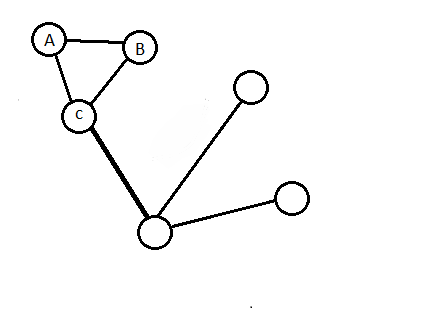
\includegraphics{Figures/triangleStruc}
	\caption{Examples of triangles in networks} 
	\label{fig:triangleStruc}
\end{figure}


For data diffusion and seed selection, this would mean that picking nodes that are neighbor to each other, would have a smaller spread then picking two not neighboring vertices. By picking two nodes that are connected to each other, they would likely share common neighbors and thus having a smaller reach.  

\subsection{Degree distribution} \label{degreeDis}
As mentioned earlier, each node have a degree. The degree distribution shows how the different degrees in the network is distributed. From the degree distribution we can see how many nodes have specific degree. Different networks have different shaped degree distribution.

For random graphs, the distribution would most likely be a Poiison distribution or binomial. For social graph, the degree distribution is often in the shape of exponential distribution. For the information diffusion, this distribution shows us how many high degree nodes there are in the network and those node would likely be high prioritized node. One of the algorithm uses the distribution to select the seed nodes. We will discuss this in later sections.  


\subsection{Degree correlations} \label{degreeCorr}
As mentioned in section \ref{degreeDis}, the network have a degree distribution with few high degree nodes and many low degree nodes. One interesting properties is the degree correlations. Degree correlations is how the high degree and low degree nodes connects to each other. One question is wether high degree nodes tends to connect to other high degree nodes, or if they prefer to connect to low degree nodes. It turns out that both incidents ar found in networks \cite{complexNetwork2003}. Most social networks are assortative, meaning vertices have a selective linking, where high degree vertex tends to connects to other high degree vertex, while technological network and biological network are most likely disassortative \cite{AssortativeMixing2002}. 

For data diffusion, this kind of behavior would result in wasting a seed by picking a majority of high degree nodes for starting seed, since most of them would be connected to each other. One solution is by mixing the selection, choose some percentage to be high degree, and some with lower degree.

\subsection{Network resilience}
For most network model, there is the need to remove nodes from the network. Removal of a node can have no effect on the network, or it can be devastating. Network resilience looks at how the network can resist to such a removal. There are two different removal schemes, the random removal where nodes are randomly picked and removed, or the targeted removal where specific nodes are removed depending on the criteria. 

The experiment mentioned in  \cite{complexNetwork2003} by Albert et al showed that for a subset of network representing the internet and the world wide web, targeted removal had a larger impact then random removal. The targeted removal removed the highest degree nodes from the network, and the random removal removed nodes randomly. The random removal had a minimal effect on the network, while the targeted removal had a much larger impact, in which mean vertex-vertex distance increased. They proposed that the internet was highly resilient to random removal, while much more vulnerable to targeted removal. 

There are other studies that proposed a different interpretation regarding the data found.	

In an example of information diffusion, a targeted removal would result in massive change to the diffusion path. By removing high degree node it would result in remove influential nodes and limit the spread of the data. Removing important nodes connectiong two different communities would result in isolation and no path towards other communities. For our case, we assume that the network is a static, unchanging network. 

\subsection{Community structure}
One properties that is often observed in a social network, is the community structure. The community structure is where a group of vertices having high density of edges with each other, while having low density of edges to other "community". We can see an example of the community structure clearly displayed from  \cite{RaceInSchool}. Where we can see the playground was divided into different groups.

This type of community structure would have a large impact on how the algorithm would select a seed for information diffusion. If all the seed would be selected in one community, the probability of spreading over to other communities would be smaller. This is of course dependent on how many intercommunity connections there are in the network.

\section{Breadth First search}
Breadth first search is an tree traversal algorithm. BFS start at the root node \textit{$v_r$}. The algorithm then stores all $v_r$s children node in an \textit{queue}. The algorithm then takes the first node from the queue, \textit{$v_1$} and stores all the children node to \textit{$v_1$} in the back of the queue, this process continues until the queue is empty and all the nodes have been iterated over. 

Breadth first search is a common graph iteration algorithm. The breadth first search is often limited by the irregular memory access where the algorithm have to find the data stored in different spaces in the memory. As mentioned earlier, independent cascade model is one special case of the Breadth first search. Breadth first search is the independent cascade model with a 100\% chanche to activate the neighbores.


\begin{algorithm}
\caption{Breadth First Search}
\begin{algorithmic}[1]
\State{$dist[\forall \textit{v} \in V] = -1; currentQ, nextQ = \oldemptyset$}
\State $step = 0; dist[root] = step$
\State ENQUEUE(nextQ,root)
\While {$nextQ\neq \oldemptyset $}
\State $currentQ = newxtQ; nextQ = \oldemptyset$
\State $step = step+1$
\While {$currentQ \neq \oldemptyset$}
\State$ u$ = DEQUEUE(currentQ)
\For {$v \in Adj[u]$}
\If {$dist[v] == -1 $}
\State $dist[v] = step$
\State ENQUEUE(nextQ, v)
\EndIf
\EndFor
\EndWhile
\EndWhile
\Return dist
\end{algorithmic}
\end{algorithm}


\section{Data diffusion}
Data diffusion is looking at how information is propagated through a network or a graph. Some example would be how a new Internet meme, a new product or how a new disease is spread through a community. The process consist of a set of starter nodes, which we will call seed nodes, that are "infected". During each time-step, there are a percentage $p_g$ that the "infected" nodes would "infect" its neighbors. Seed nodes is a set of $k$ nodes that in the initial time-step are infected. They will pass on the information/infection during each time-step and the information/infection will propagate through the network. 
 
\section{Basic Diffusion Models}
When we talk about data diffusion, we can look at how diseases or technological innovations would spread through a social network. We can simulate those kind of behaviors with different diffusion models. There are two basic diffusion models used to simulate the propagation of information through a network \cite{MaximizeSpread2003}, the \textit{linear threshold model}(LTM) and the \textit{independent cascade model}(ICM) \cite{MaximizeSpread2003}.

This process is similar to how a new product is promoted via social media. Each node is a person that can either buy the new product(activated), or ignore it(inactive). Each person will then see their friends promote the new product and potentially buy the promoted product. There are several different criteria for each person to buy the product(activates). They can either have a percentage chance to be affected by the advertisement(ICM), or they will only be interested if a percentage of his or hers friends have promoted it(LTM). Some people might have a larger circle of friends then others(high degree), while others have larger impact on a person(large $p_x$). Some might be harder to promote too(weighted edges), while some users have no friends(singletons). The different models we will focus on, are the independent cascade model and the linear threshold model.

\section{Linear threshold model}
The linear threshold model uses a threshold $\theta_v$ between the interval [0,1], which represent the fraction of $\textit{v}'s$ neighbors that need to be active to activate node $\textit{v}$, this is known as the weight of v, $b_v$. In this case, let's assume that the weight of all the nodes in this model are 0.5, meaning over half of its neighbors must be activated for the node to be activated. As we can see in Figure \ref{fig:linearThresh}, current node {\textit v} will get activated when $b_v <= \theta_v$. In figure \ref{fig:;omearThresh2} we can see that $v$ is now activated. The next time-step, Figure \ref{fig:linearThresh3}, node $w$ is checking if it will too, be activated. We can see here that $b_w !<= \theta_v$, so node $w$ will not be activated.  

We can look at the linear threshold model as a cosmetic company trying to promote their new product via social media. Each users of the product would display the new cosmetic product through social media. Each users would then be exposed to the product through their friends update. Each user would adopt the new product after seeing a percentage of their friends using the product. 

\begin{figure}[!ht]
	\begin{subfigure}{0.3\textwidth}
		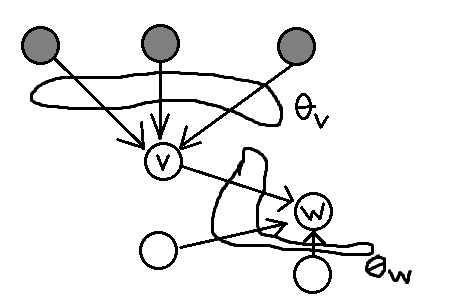
\includegraphics[width=\textwidth]{Figures/linearThreshold}
		\caption{Step 1 } 
		\label{fig:linearThresh}
	\end{subfigure}
	\begin{subfigure}{0.3\textwidth}
		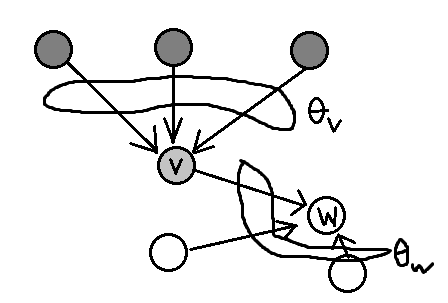
\includegraphics[width=\textwidth]{Figures/linearThreshold2}
		\caption{step 2 } 
		\label{fig:linearThresh2}
	\end{subfigure}
	\begin{subfigure}{0.3\textwidth}
		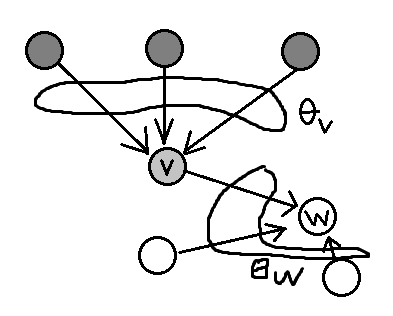
\includegraphics[width=\textwidth]{Figures/linearThreshold3}
		\caption{step 3} 
		\label{fig:linearThresh3}
	\end{subfigure}
	\caption{Linear Threshold mode}
\end{figure}

\subsection{Independent cascade model}
The independent cascade model(ICM) have a local or global probability for determining of activation, $p_v$. In figure \ref{fig:ICM_step}, we have private probability. The probability $p_v != p_w$. In \ref{fig:ICM}, the node v is activated, during the next time-step, node v have activated three neighbors. In the next time-step \ref{fig:ICM3} node w was able to activate the blue node. For a ICM with global probability, each node would then have the same probability to activate its neighbor. As we can see from Figure \ref{fig:ICM_step}, each neighbor to v is activated individually. As in \ref{fig:ICM2}, only three nodes were activated. In ICM, each node can only try to activate the neighbor once. In figure \ref{fig:ICM2}, the node that was not activated by v, got activated in \ref{fig:ICM3} by the node w.


\begin{figure}[!ht]
	\begin{subfigure}{0.3\textwidth}
		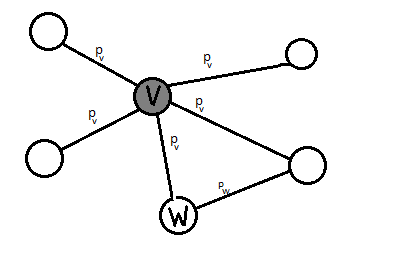
\includegraphics[width=\textwidth]{Figures/ICM}
		\caption{step 1 } 
		\label{fig:ICM}
	\end{subfigure}
	\begin{subfigure}{0.3\textwidth}
		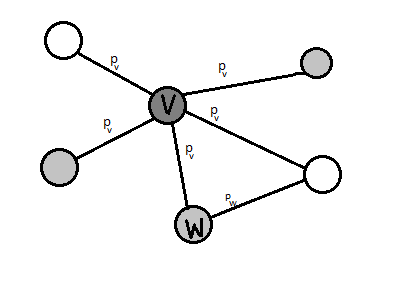
\includegraphics[width=\textwidth]{Figures/ICM2}
		\caption{step 2} 
		\label{fig:ICM2}
	\end{subfigure}
	\begin{subfigure}{0.3\textwidth}
		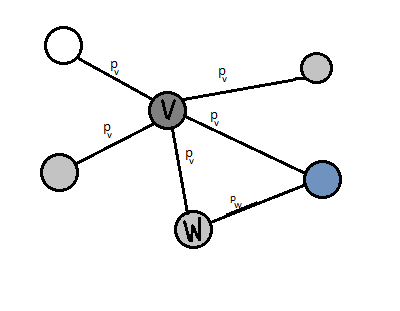
\includegraphics[width=\textwidth]{Figures/ICM3}
		\caption{step 3} 
		\label{fig:ICM3}
	\end{subfigure}
	\caption{Independent cascade model}
	\label{fig:ICM_step}
\end{figure}

We can compare the ICM with the same example we have been using, the cosmetic company promoting a product. Each new user have a chance(p$p_v$) to promote the product to a new user. The new user would then continue promoting the new product to his/hers friends. 

As mentioned earlier, the ICM is a special case of the breadth first search. If we set the transmisison probability to 1.0, meaning there are 100\% chance to activate the neighbores, the ICM is equal to BFS. BFS iterates through the graph by appending the child node not examined into the queue. Then examines a new node from the queue and repeating the process until all nodes have been examined. The main difference between the ICM and BFS, is that in ICM, there is a chance that the child node is not added into the queue. During each step, a random "coin toss" is tested to determent if the child node would be added into the queue. Other then that, both algorithms iterates through the network via edges.

\section{Matrix notations}
Nodes and edges are not the only way to present a graph, graphs and networks can be represented as sparse adjacency matrices \cite{AlgoToMath}. We can see that such an idea have been proposed in earlier literature \cite{McAndrew1963}. By representing graphs as a sparse matrix, we can often discover different ways to optimize the algorithm, we can have a different structure to store data. The adjacency matrix in particular, is a interesting way to represent the graph. A graph $G =(V,E)$, G have N vertices and M edges, this correspond to a N$\times$N adjacency matrix called A. If A(i,j)=1, then there is an edge from $v_i$ to $v_j$. Otherwise its 0. In Figure:\ref{fig:AdjaToMatrix}, we can see how a undirected graph can be represented as an adjacency matrix. To generate a undirected graph as a adjacency matrix, the matrix must be mirrored diagonally, meaning if A(i,j)=1, then A(j,i)=1, if this is not true, then the matrix would be representing a directed graph.

\subsection{Sparse Matrix}
A sparse matrix is a matrix containing few nonzero. Social graph with few edges would often be represented as a sparse matrix. Since sparse matricies only have few non-zero elements, by storing only the non-zero elements, we can have savings in memory.

\begin{figure}
	\begin{subfigure}{0.5\textwidth}
	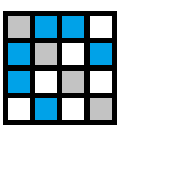
\includegraphics[width=\textwidth]{Figures/AdjacencyM}
	\caption{The adjacency matrix}
	\label{fig:AdjacencyM}
	\end{subfigure}
	\begin{subfigure}{0.5\textwidth}
	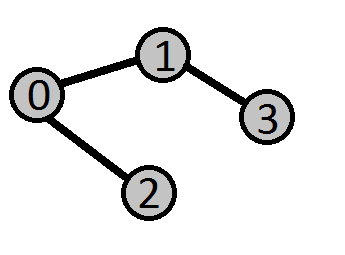
\includegraphics[width=\textwidth]{Figures/simpleGraph}
	\caption{The graph corresponding to the adjacency matrix}
	\label{fig:matrix}
	\end{subfigure}
 	\caption{Sparse matrix to graph}
 	\label{AdjaToMatrix}
\end{figure}

\subsection{Breadth First Search as a matrix multiplication.} \label{BFS as Matrix}
From  \cite{AlgoToMath}, we can see that BFS can be recast as algebraic operations. BFS can be performed by applying matrix-vector multiplication over Boolean semirings \cite{HybridBFS2015}. The graph is represented as a adjacency matrix A, then for the root node, a vector x(root)=1 is multiplied with the matrix A. $A \times x_0 = y_0$. $y_0$ is the result after the first matrix-vector multiplication and in the next iteration, $x_1 = y_0$. We can see from the Figure\ref{fig:bfsMatrix}

\begin{figure}
	
	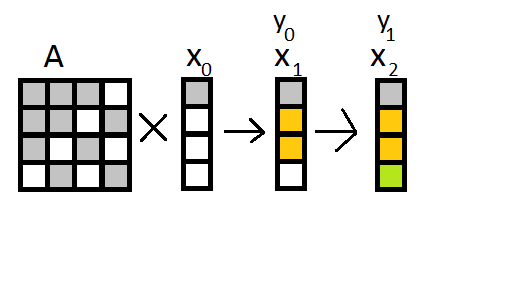
\includegraphics[width=\textwidth]{Figures/BFS_algo}
	\caption{BFS on Boolean semiring}
	\label{fig:bfsMatrix}
\end{figure}



\subsection{Semiring}
A $semiring$ is a set of elements with two binary operations. The two operations are often known as "addition"(+) and "multiplication"($\times$).  As we shown in previous section, the algorithm perform matrix multiplication uses the two operations, multiplications and addition. In  \cite{HybridBFS2015}, the AND and OR operator was chosen instead of the normal addition and multiplication. 


\subsection{BFS to data diffusion}
As mentioned before, ICM is a special case of the breadth first search. By modifying the algorithm proposed earlier, we can in theory perform ICM with matrix-vector multiplication.  

\section{Seed selection algorithm}
The seed selection algorithm, is the algorithm used to select the initial $k$ seed nodes to be chosen at the start of the information diffusion. Each selected nodes is in the initial timestep activated. During each timestep, the seed nodes will propagate the activation along the network depend on what diffusion model is used. We can compare it to a new gadget or a cosmetic company trying to promote a new product. By selecting a few influential persons to give a free sample, the new trend would most likely  spread through $viral$ $marketing$ \cite{ViralMarketing}. The seed selection algorithm would be the algorithm to select the few influential individuals to receive this free sample. There are multiple different scheme to choose from, in this section, we will focus on four different algorithms, greedy algorithm, degree algorithm, random algorithm and the independent greedy algorithm.

\subsection{The greedy algorithm}
The greedy algorithm \cite{greedyInfluenc2005} proposed by Kempe et al, is known to be the best algorithm according to the result from  \cite{greedyInfluenc2005}. The greedy algotihm starts by itterate over the entire network and finds one node that have the largest coverage and stores that node in the set $A$. The algorith then activates that node from A, and computes the coverage of each node in the network with the previous choosen node. After the algorithm finds the second node, that node is stored in A with the previous node and we have now choosen two seed node. The algorithm continues until we have choosen \textit{k} seed nodes, where each have been tested to have maximum coverage in relation with the previous choosen nodes. To compute the maximum coverage, the algorithm have to test every combination of nodes together, this results in heavy computation and the algorithm would therefore not scale well.

We can look at the greedy algorithm as a special case of BFS with a transistion probability. Each node in the network will be choosen as the seed node for the

 \begin{algorithm}
\caption{Greedy Algorithm}
\begin{algorithmic}[1]
\State Start with $A = \oldemptyset$
\While{$|A| \leq l$}
\State For each node $x$, use repeated sampling to approximate $\sigma(A \cup {x}) $ to within ($1 \pm \varepsilon$) with probability
$1 − \delta$
\State Add the node with largest estimate for $\sigma(A \cup {x})$ to A.
\EndWhile
\State Output the set $A$ of nodes.
\end{algorithmic}
\end{algorithm}

\subsection{The degree algorithm}
Another popular algorithm is the degree algorithm \cite{greedyInfluenc2005}. Unlike the greedy algorithm, does not compute the coverage of node, the algorithm picks the top \textit{k} nodes according to the degree distribution instead. The node chooses the top \textit{k} nodes with the highest degree and stores them as the seed nodes. This approach benefits over the greedy algorithm by not having as much computation time as the greedy algorithm since only one itteration is needed to compute the degree to node. The disadvantage is that this algorithm does not take the degree correlation into acount. As mentioned in section \ref{degreeCorr}, high degree nodes would often have common node as neighbor. This would result in multiple overlapping activated node choosen.

\begin{algorithm}
\caption{Degree Algorithm}
\begin{algorithmic}[1]
\State Start with $A = \oldemptyset$
\While{$|A| \leq l$}
\State For each node $x$, use repeated sampling to compute DegreeMax($x$).
\State Add the node with largest degree to A.
\EndWhile
\State Output the set $A$ of nodes.
\end{algorithmic}
\end{algorithm}

\subsection{Independent algorithm}
Another algorithm is the independent greedy algorithm. The algorithm iterates through the network, computing the spread of each node. The algorithm then chooses the vertex with the largest coverage independent of the other previous chosen nodes. This algorithm is a special case of the greedy algorithm mentioned above.

\begin{algorithm}
\caption{Independent Algorithm}
\begin{algorithmic}[1]
\State Start with $A = \oldemptyset$
\While{$|A| \leq l$}
\State For each node $x$, use repeated sampling to approximate $\sigma(A \cup {x}) $ to within ($1 \pm \varepsilon$) with probability
$1 − \delta$
\State Add the node with largest estimate for $\sigma({x})$ to A.
\EndWhile
\State Output the set $A$ of nodes.
\end{algorithmic}
\end{algorithm}


\subsection{Random algorithm}
The last one is the random algorithm. The random algorithm just picks a random seed node. This approach is the simplest to implement and easiest. The downside is that this is random and there are no strategic choosing of seed node. 

\section{RMat}
One problem during graph analyzation and calculation is finding suitable graphs to analyses. Generate graphs with desired properties is not easy to do. One solution proposed by Chakrabartiy et al is to use the "recursive matrix" or R-mat model. The R-mat model generates graph with only a few parameters, the generated graph will naturally have the small world properties and follows the laws of normal graphs, and have a quick generation speed \cite{Rmat2004}. The R-mat models goal is to generate graphs that matches the degree distribution, exhibits a " community " structure and have a small diameter and matches other criteria. \cite{Rmat2004}. The algorithm to generate such a recursive matrix is as follows: The idea is to partition the adjacency matrix into four equally sized part branded A,B,C,D, as shown in Figure\ref{fig:flipDiagonal}. The adjacency matrix starts by having all element set to 0. Each new edge is "dropped" onto the adjacency matrix. Which section the edge would be placed in, is chosen randomly. Each section have a probability of $\textit{a, b, c, d}$, and $a + b + c + d = 1$. After a section is chosen, the partition that was chosen is partitioned again. This continues until the chosen section is a 1x1 square and the edge is dropped there. From the algorithm, we can see that the R-mat generator are capable to generate graphs with total numbers of node $ \textit{V} = 2^x$. Since the algorithm partitioned the matrix into four part. This is approach would only generate a directed graph. To generate undirected graph, $b = c$ and the adjacency matrix must make a "copy flip" on the diagonal elements, like Figure \ref{fig:flipDiagonal}. 


\begin{figure}
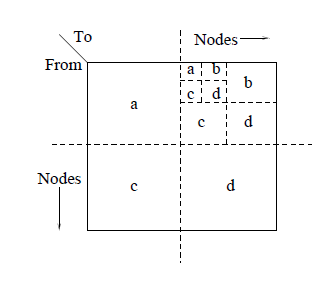
\includegraphics{Figures/Rmat}
\caption{The R-mat model \cite{Rmat2004}}
\label{fig:Rmat}
\end{figure}

\begin{figure}
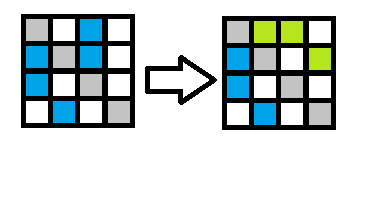
\includegraphics{Figures/flip_matrix}
\caption{How the adjacency matrix is flipped on the diagonal}
\label{fig:flipDiagonal}

\end{figure}



\begin{list}{1}
\item what is Information diffusion
\item what is the solution(bfs)
\item what is ICM
\item how to implement bfs as SpMV
\item how to apply information diffusion to bfs and problem
\item 
\end{list}


\section{High Level Synthesis}
\cite{HLSTutorial}
High Level Synthesis converst algorithms implemented on higher level down to \textit{Register Transfer Level}. It converst C and C++ codes to Verilog and VHDL. The concept of HLS was first proposed in the mid-1990 to 2000\cite{HLSTutorial}. The poor Quality of result, and lacing of tools,

%mentione register transfer level(RTL) 

\section{Memory Mapped axi interface}
Something something mapped to memory.

\section{Cache coherency }
Cache coherency, which is where multiple cache reference the same area.

\section{code}
bøalkdf


\section{ZedBoard}

We choose to implement on the zedobard